Cílem této práce bylo vytvořit aplikaci pro usnadnění seznámení se
s~virtuální realitou návštěvníkům herny a~usnadnění práce obsluze zaměstnancům herny.

Byly provedeny analýzy existujících řešení výuky a~spouštěčů. Bylo také
pozorováno chování návštěvníků a~obsluhy v~herně virtuální reality.
Výsledkem analytické části bylo mimo jiné i stanovení funkčních a
nefunkčních požadavků.

Na základě výsledků analýzy pak byla navržena aplikace pro virtuální
realitu skládající se z~dvou částí --- z~výuky ovládání systému a
spouštěče VR~aplikací.

Implementaci navržené aplikace předcházelo ověření korektnosti
navržených funkcionalit principem Proof of Concept, který poukázal na
budoucí komplikace. Jako největší komplikace se ukázalo odchýlení od
rozsahu implementace v~podobě nutnosti přidat další komponentu, a~to
malý program, tzv. agent, mající na starosti zobrazení spouštěče po
ukončení cizí VR~aplikace.

Samotná aplikace byla implementována v~jazyce \emph{C\#} s~využitím herního
engine \emph{Unity}. Součástí implementace bylo zpracování vizuálu, tvorba
prostředí, nadabování průvodce a~programování logiky aplikace.

Nakonec byla aplikace otestována v~reálném prostředí herny virtuální
reality. Testování odhalilo několik technických nedostatků ale obecně
potvrdilo funkčnost výuky. Na základě nahlášených chyb pak byla aplikace
opravena.

Realizaci aplikace lze označit za zdárnou. Lze na ní jistě spatřit
následky časové limitace. Velmi omezující byla také nemožnost spouštět
aplikaci na VR~systému okamžitě. Vlastní headset je pro studenta
finančně velmi náročná záležitost a~tak bylo nutné aplikaci testovat
pouze nárazově způsobem, kdy byla do herny přinesen zkompilovaný
binární program, otestována, chyby zaznamenány a~posléze opraveny.

\begin{figure}[h!]
\centering
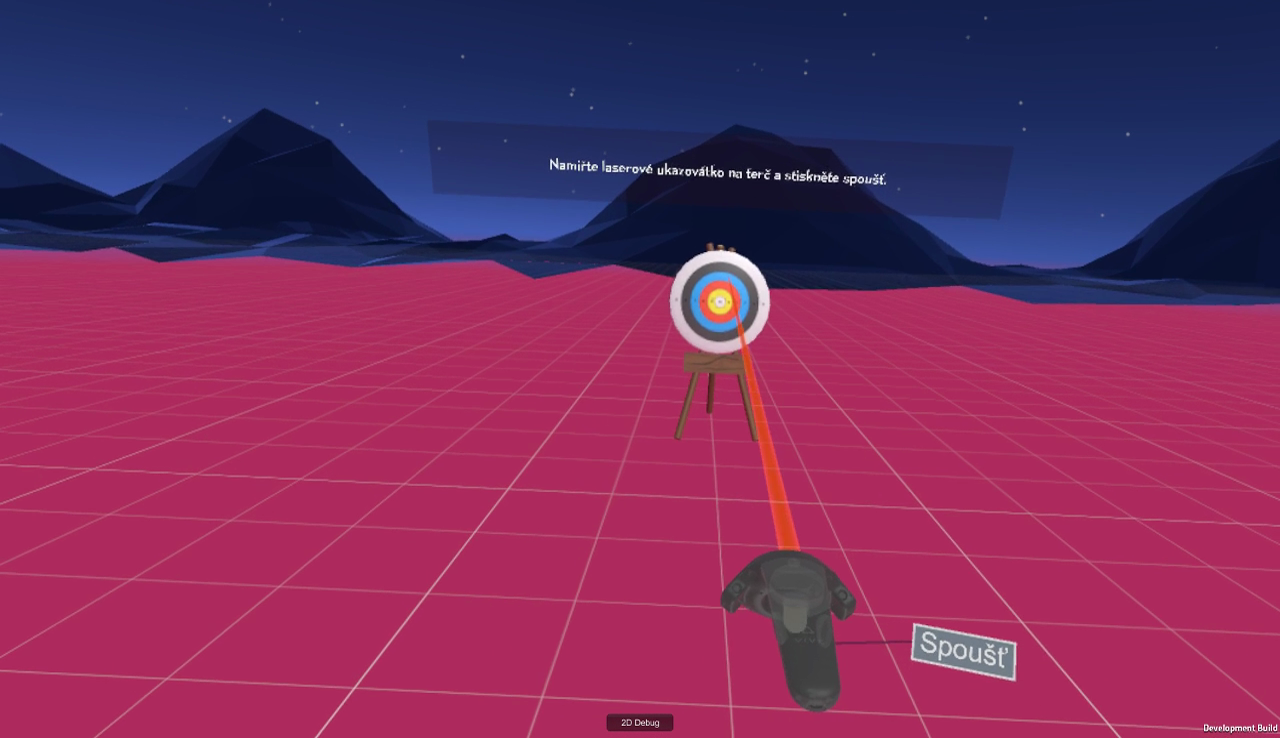
\includegraphics[width=12cm]{src/assets/result.png}
\caption{Snímek výsledné podoby aplikace}
\end{figure}

\section{Možnosti dalšího
vývoje}\label{moux17enosti-dalux161uxedho-vuxfdvoje}

Až v~průběhu realizace se naskytly zajímavé možnosti a~nápady, jak
aplikaci rozšířit. Bohužel kvůli časové limitaci nejsou součástí této
závěrečné práce, nicméně jsou uvedeny v~závěru jako příležitosti, jak
aplikaci dále rozšířit a~vyvinout.

Knihovna \emph{OpenVR} je mnohem mocnější, než je na několik prvních pohledů
zjevné. Za vinu to ovšem lze s~čistým svědomím klást špatné dokumentaci \autocite{openvrdocs},
která je nekompletní, nepřehledná a~práce s~ní není příjemná. Pokud by
se s~knihovnou pracovalo na hlubší úrovni a~doplnila se dokumentace,
bylo by teoreticky možné vyřešit několik problémů, na které se při práci narazilo.

Především by mělo být možné nahradit celý \emph{SteamVR Dashboard} a
nedovolit tak zákazníkům přístup k~platformě Steam, což by mohlo být pro
herny bezpečnější. Systém virtuální reality by tak mohl pracovat
v~kiosk módu\footnote{Kiosk mód je termín používaný pro informační systémy umístěné na veřejných místech. Jsou konfigurovány tak, aby se uživatelům zabránilo modifikaci či poškození systému.}. 

Dále je z~nezdokumentovaného kódu zjevné, že
v~knihovně existují některé metody pro stahování nainstalovaných VR
aplikací v~počítači \autocite{openvrhidden}. Znamenalo by to možnost zobrazit instalované aplikace
nejen z~platformy Steam, ale i z~platformy \emph{Oculus}, či \emph{Viveport}. Pro
účely této závěrečné práce lze však konstatovat, že výsledek nebyl o~nic
připraven, jelikož se na platformě \emph{Oculus} nenacházejí žádné aplikace
určené pro systém \emph{HTC Vive} a~platforma \emph{Viveport} není v~Evropě příliš
populární. Je cílena spíše na asijský trh. \autocite{viveportasia}

Další zajímavou funkcí by mohlo být jednodušší navázání hry pro více
hráčů. V~herně se nacházejí dva systémy \emph{HTC Vive} a~mezi návštěvníky je
oblíbená i hra se spoluhráčem. Také mřížka aplikací by mohla být vylepšena
o~doplnění řazení, kupříkladu podle oblíbenosti, určené podle doby, kterou
návštěvníci s~aplikací strávili.

Více návrhů na vylepšení aplikace může vzniknout každodenním používáním
v~herně po produkčním nasazení.
